%%%
%%%  ___ _                     __  __ _           _
%%% | _ |_)__ _ _ _  __ __ _  |  \/  (_)_  _ __ _| |__  ___
%%% | _ \ / _` | ' \/ _/ _` | | |\/| | | || / _` | '_ \/ -_)
%%% |___/_\__,_|_||_\__\__,_| |_|  |_|_|\_, \__,_|_.__/\___|
%%%                                     |__/
%%%
%%% PROJETO DE TCC: Documento modelo em LaTeX, padrão ABNT usando ABNTeX2
%%%
%%% ----------------------------------------------------------------------------
%%%
%%% Para compilar, na linha de comando:
%%%
%%%
%%%    latexmk -lualatex skeleton_tcc_proj.tex
%%%
%%% ----------------------------------------------------------------------------
%%%
%%% By Cantão! <rfcantao@gmail.com>
%%% Baseado em template do Prof. James A. Souza
%%%

\documentclass[12pt,oneside,brazil,hidelinks,article,sumario=tradicional,a4paper]{abntex2}

% Pacotes padrão da American Mathematical Society
\usepackage{amsmath}
\usepackage{amssymb}
\usepackage{mathtools}
\usepackage{indentfirst}

%%%
%%% São usadas as fontes:
%%% - Crimsom Pro: texto principal
%%% - Noto Sans: sem serifa, usada nas seções, subseções, etc
%%% - DejaVu Sans Mono: monoespaçada para listagems, URLs, etc
%%%
\usepackage{fontspec}
% CrimsonText é similar à Minion Pro, que é comercial
\setmainfont{CrimsonPro}[
  Path           = ./fonts/,
  Extension      = .ttf,
  UprightFont    = *-Regular,
  BoldFont       = *-Bold,
  ItalicFont     = *-Italic,
  BoldItalicFont = *-BoldItalic,
  SmallCapsFont  = AlegreyaSC-Regular
]
% NotoSans é similar à Myriad Pro, que é comercial
\setsansfont{NotoSans}[
  Path           = ./fonts/,
  Extension      = .ttf,
  UprightFont    = *-Regular,
  BoldFont       = *-Bold,
  ItalicFont     = *-Italic,
  BoldItalicFont = *-BoldItalic
]
\setmonofont{DejaVuSansMono}[
  Path           = ./fonts/,
  Extension      = .ttf,
  UprightFont    = *,
  BoldFont       = *-Bold,
  ItalicFont     = *-Oblique,
  BoldItalicFont = *-BoldOblique,
  Scale          = MatchLowercase
]

\usepackage[math-style=TeX]{unicode-math}
\setmathfont{Asana-Math.otf}[Scale=MatchLowercase]
%\setmathfont{STIXTwoMath-Regular.otf}[Scale=MatchLowercase]
%\setmathfont{texgyredejavu-math.otf}[Scale=MatchLowercase]


%%%
%%% Idiomas: Português e Inglês
%%%
%%% Certifique-se de ter os pacotes corretos (GNU/Linux):
%%%   sudo apt install texlive-lang-en texlive-lang-portuguese texlive-xetex
%%%
%%% O TeXLive (recomendo no caso do Windows) em geral já tem esses pacotes instalados
%%%
\usepackage{polyglossia}
\setmainlanguage{portuges}
\setotherlanguage{english}
\usepackage{csquotes}

%%%
%%% Outros pacotes úteis
%%%
\usepackage{graphicx}  % Figuras em vários formatos (png, pdf)
\usepackage{color}     % Cores
\usepackage{pgfgantt}  % Cronogramas
\usepackage{multicol}  % Documentos com várias colunas
\usepackage{booktabs}  % Tabelas profissionais
\usepackage[final]{microtype}
\usepackage{siunitx}   % Pacote para unidades físicas (recomendo muito!)
\sisetup{output-decimal-marker={,}}
\sisetup{mode=text}
\usepackage{braket}
\usepackage{makecell}
\usepackage{tikz}

\usetikzlibrary{angles,matrix,arrows.meta,calc,positioning,intersections,shadows,quotes}

%%%
%%% CORES MANEIRÍSSIMAS
%%%
\definecolor{green}{RGB}{174,226,57}    % colourlovers.com/palette/46688/fresh_cut_day (atomic bikini)
\definecolor{yellow}{RGB}{237,229,116}  % colourlovers.com/palette/937624/Dance_To_Forget (Give Your Heart)
\definecolor{orange}{RGB}{255,164,70}   % colourlovers.com/palette/1107950/Indecent_Proposal (exotic orange)
\definecolor{onlyorange}{RGB}{191,77,40}% colourlovers.com/palette/953498/Headache (Only Orange)
\definecolor{cyan}{RGB}{108,243,213}    % colourlovers.com/palette/940927/Acused (wrong cyan)
\definecolor{red}{RGB}{199,8,8}         % colourlovers.com/palette/79468/LipstickOnHisCollar (Flagged Down)
\definecolor{melon}{RGB}{209,49,92}     % colourlovers.com/palette/2350697/This_is_for_YOU! (melon)
\definecolor{blue}{RGB}{62,122,162}     % colourlovers.com/palette/794774/be_here_for_me (kreuger)
\definecolor{berry}{RGB}{95,13,59}      % colourlovers.com/palette/117122/BurberryTenderTouch (BurberryTender)
\definecolor{violet}{RGB}{87,30,240}    % From the original template (Violet Thanos)
\definecolor{hymnroyale}{RGB}{42,4,72}  % colourlovers.com/palette/81885/Hymn_For_My_Soul (Hymn Royale)
\definecolor{think}{HTML}{607848}       % colourlovers.com/palette/38562/Hands_On
\definecolor{gray}{HTML}{444444}
\definecolor{intelligentsia}{RGB}{7,69,111} % colourlovers.com/palette/4792400/Intelligentsia (Intelligentsia circle)

\usepackage{tcolorbox}
\tcbuselibrary{many}
\tcbuselibrary{theorems}

\tikzset{%
  eixos/.style={draw=black!80,text=black!80,arrows=-{Latex[width=4pt,length=6pt]}},
  eixos sem flecha/.style={draw=black!80,text=black!80},
  eixos fantasma/.style={draw=black!20,text=black!60,arrows=-{Latex[width=4pt,length=6pt]}},
  vetor/.style={draw=blue!80,text=blue!80,cap=round,arrows=-{Triangle[width=5pt,length=7pt]},very thick},
  linhaforte/.style={draw=#1,ultra thick,cap=round},
  linhamedia/.style={draw=#1,thick,cap=round},
  ponto/.style={fill=#1!40,draw=#1,semithick,inner sep=2pt,circle},
  projecao/.style={draw=#1,densely dotted,thick},
  projecao 2/.style={draw=#1,densely dash dot,thin},
  etiqueta/.style n args={3}{text=#1,draw=#2,fill=#3,solid,font=\scriptsize,inner sep=2pt,minimum height=13pt,drop shadow={opacity=0.8,shadow xshift=.3ex,shadow yshift=-.3ex}},
  face/.style={draw=black,fill=white,thick,cap=round},
  blocoq/.style={very thick,draw=black!70,fill=black!5,inner sep=8pt,align=center,drop shadow={opacity=0.8,shadow xshift=.3ex,shadow yshift=-.3ex}},
  blocor/.style={very thick,draw=red!20,fill=red!5,inner sep=8pt,align=center,rounded corners,drop shadow={opacity=0.8,shadow xshift=.3ex,shadow yshift=-.3ex}},
  blococ/.style={very thick,draw=green!20,ellipse,fill=green!5,inner sep=8pt,align=center,rounded corners,drop shadow={opacity=0.8,shadow xshift=.3ex,shadow yshift=-.3ex}},
  conecta/.style={draw=black!50,text=black!80,cap=round,arrows=-{Triangle[width=5pt,length=7pt]},thick},
  labelst/.style={label distance=-6pt,font=\scriptsize\scshape,align=center,black!80,inner sep=2pt}
}

\newtcbtheorem[number within=section]{theo}{Teorema}{
  enhanced,
  %skin=bicolor,
  arc=0mm,
  colback=black!3,
  colframe=black!50,
  colbacktitle=white,
  colbacklower=white,
  coltitle=black,
  fonttitle=\small,
  toptitle=3pt,
  bottomtitle=3pt,
  top=5pt,
  bottom=5pt,
  left=10pt,
  right=10pt,
  boxrule=0pt,
  titlerule=0pt}{th}

%%%
%%% Informações do PDF
%%%
\makeatletter
\hypersetup{%
  pdftitle={\@title},
  pdfauthor={\@author},
  pdfsubject={\imprimirpreambulo},
  pdfcreator={LuaLaTeX with abnTeX2},
  pdfkeywords={tcc}{licenciatura em física}{projeto de pesquisa},
  colorlinks=true,    % false: boxed links; true: colored links
  linkcolor=gray,     % color of internal links
  citecolor=gray,     % color of links to bibliography
  filecolor=gray,     % color of file links
  urlcolor=gray,
  bookmarksdepth=4
}
\makeatother

%%%
%%% Bibliografia
%%%
%%% Aqui estamos usando por padrão um programa chamado 'biber'. Ele é o responsável
%%% por converter o arquivo 'skeleton.bib' nas referências formatadas no padrão
%%% ABNT.
%%%
%%% Para saber mais:
%%% https://www.overleaf.com/learn/latex/Bibliography_management_in_LaTeX
%%%
\usepackage[backend=biber,style=abnt,noslsn,repeatfields,sccite,scbib,backref]{biblatex}
\addbibresource{./tcc.bib}

%%% Função seno em PT-BR
\DeclareMathOperator{\sen}{sen}
\DeclareMathOperator{\CNOT}{\mathbf{CNOT}}

%%%
%%% Configurações do documento para ABNTeX2
%%%
\titulo{TRANSMISSÃO DE INFORMAÇÃO QUÂNTICA: SIMULAÇÃO DE RUÍDOS NO FENÔMENO DE TELETRANSPORTE QUÂNTICO}
\autor{Bianca Miyabe Santos Freitas}
\orientador{Prof. Dr. Renato Fernandes Cantão}
\instituicao{%
  UNIVERSIDADE FEDERAL DE SÃO CARLOS --- \textsl{CAMPUS} SOROCABA
  \par
  CENTRO DE CIÊNCIAS E TECNOLOGIAS PARA A SUSTENTABILIDADE
  \par
  DEPARTAMENTO DE FÍSICA, QUÍMICA E MATEMÁTICA}
\tipotrabalho{Projeto de Trabalho de Conclusão de Curso}
\preambulo{Projeto de Trabalho de Conclusão de curso apresentado ao curso de Licenciatura Plena em Física da Universidade Federal de São Carlos, \textsl{Campus} Sorocaba, como requisito para a conclusão da disciplina TCC 1.}
\local{Sorocaba}
\data{Abril, 2022}

% Modelo sugerido pela UFSCar
\renewcommand{\imprimircapa}{%
  \begin{capa}%
    \centering
    {\imprimirinstituicao\vfill}

    {\ABNTEXchapterfont\large\imprimirautor}

    \vfill
    {\ABNTEXchapterfont\bfseries\LARGE\imprimirtitulo}
    \vfill

    \large\imprimirlocal

    \large\imprimirdata

    \vspace*{15mm}
  \end{capa}
}

\begin{document}

%%% Elementos pré-textuais (capa, sumário, etc)
\pretextual
\imprimircapa
% \imprimirfolhaderosto

\begin{resumo} 

Com a hipótese da utilização da Mecânica Quântica para o processamento de informação, surge uma nova área de estudo a chamada Computação Quântica. Os estudos desta área remetem ao comportamento e implementação do  \textit{qubit} como unidade básica de informação. Apesar da implementação de um Computador Quântico já existir, os estudos sobre o comportamento do qubit, bem como dos mecanismos aos quais este pode se submeter se fazem necessários para o desenvolvimento de processadores com maior número e melhor qualidade destas entidades quânticas. Nesse sentido, a proposta deste trabalho consiste em elaborar uma simulação para o estudo do fenômeno de Teletransporte Quântico para a transmissão de informação quântica utilizando qubits emaranhados, bem como na verificação dos efeitos de possíveis ruídos na transmissão.


  \vspace{\onelineskip}

  \noindent
  \textbf{Palavras-chave}: Informação quântica. Teletransporte quântico. Qubit.
\end{resumo}
\newpage


%\begin{resumo}[Abstract] % Resumo em EN
%  \begin{otherlanguage*}{english}
 %   Same as above, but in English.
%    \vspace{\onelineskip}

%    \noindent
%    \textbf{Keywords}: Word 1. Word 2. Word 3.
%  \end{otherlanguage*}
%\end{resumo}
%\newpage


%%% Caso já seja um trabalho final
% \listoffigures*
% \clearpage

% \listoftables*
% \clearpage

 \tableofcontents*
 \clearpage

%%% Pular página
% \clearpage

%%% Elementos textuais (o documento em si)
\textual%

%%%
%%% INTRODUÇÃO
%%%
\section{Introdução}\label{sec:intro}


Segundo \textcite{conceitoinformação}, o conceito de informação possui seu significado cotidianamente atribuído como \textit{conhecimento comunicado}. Nesse sentido, a informação já existia nas pinturas rupestres há cerca de \num{45,5} mil anos atrás, nas quais estão registradas uma série de imagens no intuito de comunicar, seja um evento ou ainda uma quantidade. Apesar do conceito de informação aparecer desde os primórdios do estabelecimento da humanidade, é apenas na década de 1940 que esta passa a ser objeto de estudo com os trabalhos de Claude Elwood Shannon (1916--2001), que desenvolve uma teoria matemática para a informação \cite{CiênciaTransiçãoSeculosa}.

O objetivo principal da Teoria da Comunicação de Shannon ou \textit{Teoria Matemática da Comunicação} (TMC), consistiu em sistematizar o conhecimento acumulado até então, acerca da eficiência em sistemas de comunicação. A teoria descreve o funcionamento lógico-matemático de um destes sistemas, composto por um gerador de informação, um meio de transmissão e um receptor, conforme ilustra a Figura~\ref{comunicshannon} \cite{MTC}.

\begin{figure}[ht!]
  \centering
  \caption{Esquema geral de um sistema de comunicação com a Fonte de Informação criando uma Mensagem a ser transmitida pelo Transmissor que a transforma em um Sinal. Na transmissão pode haver uma Fonte de Ruído. O sinal é recebido pelo Receptor e finalmente a mensagem chega ao seu Destino.}\label{comunicshannon}
  % 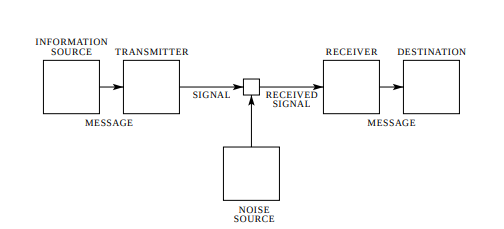
\includegraphics[width=0.65\textwidth]{comunicadorshannon.png}
  \begin{tikzpicture}
    \matrix (A) [matrix of nodes,
    column sep=25pt,
    row sep=30pt,
    nodes={minimum size=35pt}]
    {
      \node[label={[labelst]above:Fonte de\\informação},blocoq] (fonte) {}; &
      \node[label={[labelst]above:Transmissor},blocoq] (trans) {}; &
      \node[minimum size=10pt,blocoq] (conn) {}; &
      \node[label={[labelst]above:Receptor},blocoq] (rec) {}; &
      \node[label={[labelst]above:Destino},blocoq] (dest) {}; \\
      & & \node[label={[labelst]below:Fonte de \\ruído},blocoq] (ruido) {}; \\
    };
    \draw[conecta] (fonte) -- node[pos=0.5,below,labelst,yshift=-20pt] {Mensagem} (trans);
    \draw[conecta] (trans) -- node[pos=0.5,below,labelst] {Sinal} (conn);
    \draw[conecta] (conn) --  node[pos=0.5,below,labelst] {Sinal\\recebido} (rec);
    \draw[conecta] (rec) -- node[pos=0.5,below,labelst,yshift=-20pt] {Mensagem} (dest);
    \draw[conecta] (ruido) -- (conn);
  \end{tikzpicture}
  \fonte{Adaptado de \textcite[p. 380]{MTC}.}
\end{figure}

De acordo com  a TMC, um \textit{gerador de informação} é um objeto capaz de produzir um conjunto $X$ de $n$ eventos com probabilidade de ocorrência $P(X)$, enquanto um \textit{receptor} possui um conjunto $Y$, também com $n$ eventos, com probabilidades associadas $P(Y)$. Durante a transmissão é possível que parte da informação seja perdida, devido a ocorrência de ruídos, o que resulta diretamente na modificação dos valores de probabilidade dos elementos recebidos do conjunto $Y$. Reconhecendo portanto os elementos de $X$ e suas probabilidades associadas, espera-se que uma mensagem bem transmitida, ou seja, sem interferência de ruídos, seja aquela cujas probabilidades dos elementos do conjunto $Y$ sejam as mesmas dos conjunto de elementos de $X$. Assim, se essas probabilidades forem distintas, podemos concluir que houve perda de informação na transmissão \cite{mathematical}.

De maneira geral, a informação é quantificada de acordo com os recursos físicos necessários para que ela seja representada, ou seja, na capacidade de armazenamento, comunicação e representação de um conjunto $X$ de possíveis informações. Em um computador clássico, por exemplo, armazenamos informações através das unidades binárias chamadas \textit{bits}\footnote{Nome proposto, segundo o artigo original de Shannon por J.W. Turkey \cite{MTC}.}. Dessa forma, os bits são a menor unidade de armazenamento de informação em um computador de arquitetura clássica, podendo representar o estado 1 ou o estado 0 \cite{MTC}.

A combinação desses bits faz com que uma mensagem possa ser armazenada, processada ou transmitida em um computador clássico. Nesse sentido, quão maior, ou ainda, quão mais complexa for a mensagem a se operar, mais bits serão necessários e consequentemente mais recursos físicos para a representação destes. Com a evolução dos computadores e consequentemente com a necessidade de um maior número de bits a se operar, ocorreu um processo de miniaturização do hardware, em particular, do dispositivo transistor. Com transistores cada vez menores, menos espaço físico era necessário para operar a informação e cada vez mais informação era possível de ser operada simultaneamente. Basta recordar que o tamanho de um smartphone moderno é muito menor do que a primeira unidade de computador eletrônico criado, o ENIAC que ocupava um espaço de \SI{180}{\square\meter} \cite{eniac}.

Porém, em 1965 foi estabelecido por Gordon E. Moore um limite de processamento devido ao número de transistores necessários comprimidos em um pequeno espaço, versus sua dissipação de calor, o que corrompe a informação. Esse limite recebeu o nome de ``Lei de Moore''. Nela, \textcite{moore} estima que o número de transistores de um computador dobraria a cada dois anos sem que seu valor fosse alterado. Esse limite foi brevemente superado por novas tecnologias de materiais\footnote{A empresa IBM, produziu em 2014 um nanochip de silício de 7 nm e em 2015 anunciou a produção de chips de processamento com nanotubos de carbono de tamanho 1,8nm \cite{chipibm}.}, deixando evidente, entretanto, a necessidade de expandir a capacidade de processamento dos sistemas atuais, visto que a tendência de crescimento na quantidade de informação processada é cada vez maior.

Em 1981, o físico Richard Feynman, em um de seus seminários, sugeriu que os conceitos de Mecânica Quântica fossem aplicados à computação para que a informação pudesse ser operada de maneira mais rápida e em maior quantidade \cite{TeoQuanInfoEntreCopia}.

A Mecânica Quântica é o ramo da Física que surge na virada do século XX a partir de uma série de experimentos que não puderam ser explicados classicamente. As hipoteses produzidas por nomes como Planck, Eistein, Bohr e De Broglie e posteriormente complementadas por Schrödinger, Heisenberg e Dirac, descrevem uma nova área na Física. Para o desenvolvimento de um computador de arquitetura quântica, destacamos a importância do \textit{Princípio da Superposição de Estados}.

O Princípio da Superposição de Estados determina que um estado de um sistema físico é composto por todas as informações possíveis de serem extraídas dele em uma medição. Disso ocorre que um estado possui definição probabilística a partir de todos as possibilidades de ocupação deste. Esses estados são representados por um vetor do espaço complexo de Hilbert $H$, chamados também, usando a notação de Dirac, de \textit{kets} e representados por $\ket{\psi}$.

Nesse sentido, unindo a teoria quântica às necessidades de aumento no processamento de informação, surge uma nova área de estudo, a \textit{Computação Quântica}. Segundo \textcite{CompInfoQuantica} e \textcite{dwave}, a devida construção de um computador de arquitetura quântica foi precedida pelos eventos descritos a seguir:

\begin{description}
  \item[1985] David Deustch propõe matematicamente o primeiro computador quântico universal;
  \item[1994] Peter Shor cria o primeiro programa essencialmente quântico, ou seja, ele não poderia ser executado em um computador clássico. Este programa, conhecido como Algoritmo de Shor, reduziria o tempo de fatoração de números grandes de possíveis meses para apenas segundos caso fosse utilizado em um computador real de arquitetura quântica;
  \item[1999] O MIT apresenta o primeiro protótipo de um computador quântico real;
  \item[2007] A empresa D-Wave apresenta o primeiro computador essencialmente quântico.
\end{description}

A descrição da arquitetura de um computador quântico esbarra no mesmo princípio daquela de um computador clássico, ou seja, em sua unidade fundamental de armazenamento de informação. De maneira análoga ao computador clássico, que utiliza como unidade de informação o bit, o computador quântico utilizará o \textit{qubit} (ou q-bit, ou ainda, quantum bit).

Um qubit, ou bit quântico, pode ser produzido de maneiras distintas\footnote{Qubits podem ser fisicamente criados utilizando, por exemplo, spins de átomos presos em uma armadilha. Essa armadilha pode ser do tipo óptica ou até mesmo magnética. É possível também polarizar fótons para sua obtenção. A determinação do método é definida principalmente pelo mecanismo que melhor conseguir isolar o \textit{qubit}, já que este é facilmente influenciado pelo ambiente externo \cite{materialdidaticomecquantica}.}, porém nosso foco de estudo está nas suas propriedades. Um qubit é uma unidade com propriedades quânticas que atua sob o regime de superposição de estados. Isso significa que ele consegue armazenar simultaneamente mais de um estado de informação, diferente do bit clássico que armazena apenas um dos estados por vez. Decorre desta propriedade a maior capacidade de operar a informação em comparação aos mecanismos clássicos segundo apresentado na Tabela~\ref{tabelabit}.

\begin{table}[ht]
  \centering
  \caption{Comparação entre a quantidade de bits clássicos e quânticos necessários para se operar uma informação.}\label{tabelabit}
  \begin{tabular}{ccc}
    \toprule
    \thead{Quantidade \\ de bytes \\ (informação)} & \thead{Quantidade \\ de bits clássicos} & \thead{Quantidade \\ de qubits} \\
    \midrule
    1         & 8            & 3  \\
    \num{e6}  & \num{8.3e6}  & 23 \\
    \num{e12} & \num{8.8e12} & 43 \\
    \bottomrule
  \end{tabular}
  \fonte{Elaborada pelo autor.}
\end{table}

De modo a generalizar a comparação entre bits classicos e quânticos, podemos estabelecer a relação:
\begin{equation} \label{bitvsqubit}
n\, \text{qubits} = 2^{n}\,\text{bits}.
\end{equation}

Portanto, podemos concluir que menos qubits são necessários para operar a informação, em comparação ao bit clássico, o que está diretamente relacionado com a velocidade e com a capacidade de realização deste.

A descrição de um qubit consiste em uma combinação linear de dois possíveis estados quânticos $\ket{0}$ e $\ket{1}$ de modo que:
\begin{equation} \label{comblinearqubit}
 \ket{\psi} = \alpha \ket{0} + \beta \ket{1}, \quad \text{com } \alpha^{2} + \beta^{2} = 1,
\end{equation}
sendo $\alpha$ e $\beta$ as amplitudes probabilísticas dos estados quânticos $\ket{0}$ e $\ket{1}$.

É interessante observar que, apesar de qubits conseguirem armazenar mais informação devido à superposição de estados, a obtenção direta desta é impossível visto que, diferente da mecânica clássica, onde podemos observar se um bit se encontra em um estado 0 ou um estado 1, em situações quânticas a observação faz com que o sistema colapse. Portanto, o foco de aproveitamento de um qubit está em conseguir transferir a informação que ele armazena, sem que uma medida seja realizada diretamente nesta unidade quântica \cite{chuang}.

Apesar dessa aparente dificuldade em se obter a informação quântica, existem alguns mecanismos que facilitam e possibilitam sua obtenção. Segundo \textcite{materialdidaticomecquantica}, para a compreensão destes mecanismos serão necessários estabelecer alguns teoremas que regem a informação quântica.

\begin{theo}{não-clonagem}{teo1}
É impossível clonar um estado quântico, ou seja, qualquer dispositivo que receba um estado quântico como entrada, será incapaz de reproduzir como saída exatamente o mesmo estado quântico.
\end{theo}

\begin{theo}{}{teo2}
Não é possível obter um estado quântico desconhecido de um sistema único e individual realizando uma medição sobre este, independente do tipo e/ou sequência de medições que se realize.
\end{theo}

Pelos Teoremas~\ref{th:teo1} e~\ref{th:teo2} parece ser improvável a proposta de que a informação quântica se sobressaia em relação à clássica, mas é exatamente devido a eles e aos mecanismos que estes proporcionam que a informação quântica se torna tão promissora. Os mecanismos que estudaremos nesse trabalho são o \textit{Emaranhamento (ou Entrelaçamento) Quântico} e o \textit{Teletransporte Quântico}.

O Emaranhamento Quântico é uma consequência quântica proveniente da superposição de estados de elementos dessa natureza. Vale ressaltar que objetos e fenômenos quânticos nem sempre possuem o análogo clássico, como o caso de spins. Nesse fenômeno duas particulas interagem de modo que o estado quântico de uma delas não pode ser mais descrito sem o da outra. Isso faz com que, mesmo que as partículas estejam distantes uma da outra, elas continuam a compartilhar os estados quânticos. É possível portanto, que conhecendo algumas propriedades de uma das partículas, seja possível determinar esta mesma característica da outra partícula. A determinação das propriedades de uma das partículas culmina na instantânea definição na segunda, pois elas compartilham o mesmo estado quântico, o que nos leva a utilização do Emaranhamento para a realização do Teletransporte Quântico \cites{materialdidaticomecquantica}{fonzar}{TeoQuanInfoEntreCopia}.

O Teletransporte Quântico consiste em uma série de operações realizadas por intermédio de um circuito de natureza quântica que pretende enviar uma mensagem de um ponto \(A\) até um ponto \(B\). Para a realização desse procedimento, dependemos essencialmente de ao menos três qubits. Para introduzir esse conceito, iremos nos apropriar de uma história hipotética a título de esclarecer a ideia principal do fenômeno. Imagine por um instante que se deseja enviar uma fotografia para alguém que não se vê há muito tempo. Existem essencialmente duas maneiras de realizar o envio: pode-se enviar a foto pelo correio e aguardar que o destinatário a receba, processo chamado de transporte de informação, ou ainda, você poderia criar um arquivo digital com informações sobre a fotografia, de maneira que aquele que recebe o arquivo, possa de alguma maneira recriar a foto; nesse segundo caso, a foto seria teletransportada \cite{materialdidaticomecquantica}.

Trazendo a situação descrita para o universo quântico, o teletransporte de estados quânticos consiste em uma série de operações que possibilitam descrever no ponto \(B\) um estado existente no ponto \(A\). A princípio, devido ao Teorema~\ref{th:teo1} da não-clonagem\footnote{A informação clássica pode ser facilmente reproduzida, basta recordar que um livro pode ser impresso com a tiragem de exemplares desejada. Já a informação quântica não é plausível de reprodução direta. Algumas provas matemáticas desta impossibilidade são apresentadas em \textcite{TeoQuanInfoEntreCopia}.}, seria impossível ``clonar'' um qubit, ou seja, teletransportar a informação de modo semelhante ao que ocorre com um canal clássico. Porém, segundo \textcite{bennet}, é possível contornar o problema utilizando um canal de informação clássico, semelhante ao apresentado por Shannon na TMC, porém utilizando como emissor-receptor um par de partículas emaranhadas quanticamente.

Na literatura encontram-se as mais diversas explicações sobre como funciona o teletransporte quântico \cites{bennet}{experimentalqt}{zeilinger}{brassard1996teleportation}{materialdidaticomecquantica} e na maioria dos casos, os leitores são introduzidos a dois personagens: Alice e Bob.

Na história, os cientistas Alice e Bob estão localizados em dois laboratórios distintos, cada um deles possui um qubit, $q_{A}$ e $q_{B}$ e estes estão emaranhados, produzindo um estado quântico emaranhado denominado de $\ket{\psi_{AB}}$. Alice precisa enviar uma mensagem urgente para Bob utilizando um outro qubit, $q_{C}$. Portanto, no início do processo de teletransporte, Alice possui dois qubits, o que ela deseja enviar e o que possui o estado quântico emaranhado com o qubit de Bob.

Alice realiza então uma série de operações entre seus qubits e, como um deles está emaranhado com o de Bob, este saberá que algo está mudando. Para continuar o processo de teletransporte, Alice faz uma medição em seus qubits, colapsando-os e envia, via um canal clássico, a informação dos qubits colapsados para Bob. Este por sua vez, por saber qual era o estado inicial de $q_{A}$ devido ao emaranhamento, conseque reconstruir a mensagem presente originalmente no qubit $q_{C}$ enviado por Alice. Portanto, a mensagem é reconstruida e não clonada, não violando o princípio da não-clonagem (Teorema~\ref{th:teo1}). A não-clonagem fica explicitada no momento em que a medida é realizada em $q_{A}$ e $q_{C}$, colapsando-os, de modo que existe apenas uma cópia do estado de $q_{C}$ dado por $\ket{\psi_{C}}$.

O teletransporte quântico possui algumas questões que devem ser salientadas. A primeira delas é que, de fato, este é um método de transmissão de informação extremamente seguro, visto que, se o receptor não tiver o qubit emaranhado com o do emissor, a mensagem não poderá ser recuperada, além do fato de que a informação original é destruída na transmissão da mensagem. Disso decorre imediatamente a segunda questão. A informação pode, eventualmente, sofrer interferências de ruídos externos durante seu envio e por não possuir mais a mensagem original, pode ser perdida.

Portanto, o estudo dos possíveis ruídos que possam interferir no teletransporte, assim como na transmissão clássica, faz com que, mesmo que estes ocorram, seja possível recuperar a informação ao final do processo, corrigindo-os. Existem os mais diversos tipos de ruídos aos quais a mensagem pode ser exposta, o que torna praticamente impossível prever quais deles efetivamente ocorreram ao recuperar uma mensagem; porém, o estudo de ruídos familiares torna possível o reconhecimento destes tornando mais provável a recuperação da informação enviada \cite{fonzar}.

A construção do sistema de teletransporte quântico demanda um circuito onde operam as chamadas \textit{portas lógicas quânticas} e portanto, a realização experimental de um teletransporte quântico demanda efetivamente um computador de arquitetura quântica para que as operações ocorram sob os qubits. Apesar de já existirem computadores quânticos, ainda são necessários estudos acerca deste para que cada vez mais a qualidade dos qubits seja melhorada. Porém, devido aos recursos de simulação, podemos utilizar um computador de arquitetura clássica para simular tanto um qubit quanto os circuitos lógicos necessários para a realização do teletransporte quântico, a título do estudo, por exemplo, dos efeitos de ruídos na transmissão da informação quântica conforme propomos nesse trabalho.

%%%
%%% OBJETIVOS
%%%
\section{Justificativa e objetivos}\label{sec:just}

Apesar da construção de um computador de arquitetura quântica não ser mais apenas uma projeção futurista, sua efetividade ainda depende de alguns fatores. Os dois principais são o número de qubits operando simultaneamente e a qualidade destes qubits.

Quanto ao número de qubits, atualmente existe o processador \textit{Eagle} da empresa IBM, que opera com 127 qubits\footnote{O processador \textit{Eagle} foi apresentado pela IBM em Novembro de 2021 e, segundo a empresa, nos próximos anos devem ser apresentados os processadores de 433 e 1121 qubits \cite{processadoribm}.}, e também a startup QuEra que foi capaz de produzir um processador de 256 qubits \cite{quera}. Em relação à qualidade dos qubits, ou seja, na capacidade destes para a resolução de problemas reais, são necessários constantes aprimoramentos, visto que esta é uma tecnologia em ascensão.

Nesse sentido, os estudos e projetos acerca das possíveis melhorias na direção da computação quântica efetiva, são muitas vezes realizados com o auxílio de ferramentas de simulação desenvolvidas em computadores de arquitetura clássica. A utilização deste tipo de simulação se faz necessária pois não existem ainda recursos capazes de reproduzir de forma conveniente a situação que se deseja analisar, principalmente por se tratar de uma área ainda nova e em constante desenvolvimento \cite{videoyoutube}.

O objetivo principal desta proposta consiste portanto, em realizar um estudo acerca dos efeitos de possíveis ruídos no fenômeno de teletransporte quântico, utilizando uma simulação de circuitos quânticos em um computador de arquitetura clássica. Para realizar este objetivo, pretende-se:
\begin{enumerate}
  \item Definir o conceito de Teletransporte Quântico;\label{obj1}
  \item Delinear as situações onde o fenômeno é utilizado, em particular na transmissão de informação;\label{obj2}
  \item Elencar os tipos de ruídos que podem interferir na transmissão de informação durante o fenômeno;\label{obj3}
  \item Construir a simulação de comportamento de um qubit;\label{obj4}
  \item Estruturar as portas lógicas quânticas a serem simuladas para o presente estudo;\label{obj5}
  \item Estabelecer uma sequência de testes com os algoritmos de ruído;\label{obj6}
  \item Comparar os resultados obtidos na simulação desenvolvida com os resultados provenientes de simuladores em computadores de arquitetura quântica como o IBM Quantum e o Azure Quantum.\label{obj7}
\end{enumerate}

%%%
%%% METODOLOGIA
%%%
\section{Metodologia}

Para atingir os objetivos citados na Seção~\ref{sec:just}, pretende-se iniciar o desenvolvimento realizando uma revisão dos tópicos necessários de Mecânica Quântica, bem como das ferramentas matemáticas necessárias para definir conceitual e matematicamente o Teletransporte Quântico. Em linhas gerais, a compreensão da Mecânica Quântica demanda principalmente o domínio da Álgebra Linear com a notação de \textit{``bracket''} definida por Paul Dirac em 1939 \cite{DIRAC}.

Estabelecidos os conceitos necessários para a definição do fenômeno abordado, será possível delinear suas aplicações para justificar este trabalho. Nesse sentido, será necessária uma revisão bibliográfica para coletar as informações das mais recentes e promissoras aplicações do fenômeno.

Como o foco principal deste trabalho está nos estudos acerca dos efeitos de ruídos no fenômeno de Teletransporte, será necessário elencar os principais ruídos existentes para definir quais serão abordados no trabalho. Segundo \textcite{teseufscar}, os principais tipos de ruídos associados à decoerência da informação quântica, ou seja, a sua alteração do estado original são:

\begin{description}
  \item [Inversão de bit (\textit{bitflip}):] esse ruído consiste essencialmente na inversão do estado dos qubits emaranhados, fazendo com que estes saiam de um chamado estado puro --- essencial para o fenomeno de emaranhamento --- para um estado misto.
  \item [Inversão de fase (\textit{phaseflip}):] inverte a fase da função de onda que representa os qubits emaranhados.
  \item [Inversão de bit e fase (\textit{bit-phase flip}):] inverte tanto o estado quanto a fase do qubit.
\end{description}

Após os devidos estudos teóricos, pretende-se iniciar a construção da simulação. Para isso, o primeiro passo é a delimitação das ferramentas e linguagens a serem utilizadas. A escolha da linguagem de programação será o Python para este trabalho e justifica-se pelo fato de sua versatilidade e ampla implementação tanto na Física quanto nas simulações físicas.

Em seguida, pretende-se construir um algoritmo que seja capaz de simular a natureza quântica do qubit. É necessário simular, utilizando as ferramentas de Álgebra Linear, a função de onda que descreve o qubit para que este possa interagir com as portas lógicas, que também serão implementadas, no intuito de realizar, de forma puramente computacional, o fenômeno de teletransporte quântico. Serão utilizadas no fenômeno de teletransporte quântico as portas lógicas quânticas \textit{Controlled-Not} e \textit{Hadamard}.

A porta Controlled-Not, ou apenas \(\CNOT\), essencialmente opera entre dois qubits, sendo um deles de controle e o outro o qubit alvo. Ao passar por essa porta o qubit alvo sofrerá ou não uma inversão de fase dependendo do estado do qubit de controle. Esta porta pode ser representada matematicamente utilizando a matriz:
\begin{equation}\label{CNOTMATRIX}
  \mathbf{CNOT}=\begin{bmatrix}
                  1 & 0 & 0 & 0\\
                  0 & 1 & 0 & 0\\
                  0 & 0 & 0 & 1\\
                  0 & 0 & 1 & 0
                \end{bmatrix}.
              \end{equation}

Já a porta Hadamard, atua em apenas um qubit e possui como objetivo rotacioná-lo para que, ao invés de atuar sob as bases do espaço de Hilbert $\ket{0}$ e $\ket{1}$, estes passem a ser $\frac{\ket{0} + \ket{1}}{\sqrt{2}}$ e $\frac{\ket{0} - \ket{1}}{\sqrt{2}}$. Essa transformação essencialmente faz com que os qubits agora possuam chances iguais de colapsarem em \(0\) ou \(1\) quando medidos. A representação matemática da porta Hadamard é descrita por:
\begin{equation}\label{HADAMARDMATRIX}
  \mathbf{H}= \frac{1}{\sqrt{2}}\begin{bmatrix*}[r]
                                  1 & 1 \\
                                  1 & -1
                                \end{bmatrix*}
                              \end{equation}

Construídos os algoritmos que simularão o qubit, as portas lógicas e o fenômeno de Teletransporte, será necessária a execução de uma série de testes para a avaliação dos resultados obtidos. Para tal, pretende-se utilizar o IBM Quantum Tools o laboratório online de ferramentas quânticas que disponibiliza ferramentas de construção de código e circuitos que são operados diretamente em seu computador quântico. Portanto, será possível obter o comportamento das medidas esperadas em nossa simulação, diretamente de um computador de arquitetura quântica, tornando a comparação dos resultados mais consistente.

%%%
%%% CRONOGRAMA
%%%
\section{Cronograma de Atividades}


\begin{table}[ht!]
  \begin{center}
    \caption{Cronograma de desenvolvimento do Trabalho de Conclusão de Curso. Cada linha corresponde a um objetivo específico da Seção~\ref{sec:just}. Cada coluna
      corresponde a um mês de Maio a Setembro de 2022.}\label{tab:cronog}
    \begin{ganttchart}[hgrid,
                       vgrid,
                       bar/.append style={fill=blue!10,draw=blue},
                       bar top shift=0.1,
                       bar height=0.8,
                       x unit=20mm,
                       y unit chart=6mm]{1}{5}
     \gantttitle{Meses}{5} \\
     \gantttitlelist{1,...,5}{1} \\
      \ganttbar{\ref{obj1}}{1}{2}\\
      \ganttbar{\ref{obj2}}{2}{2}  \\
      \ganttbar{\ref{obj3}}{2}{2} \\
      \ganttbar{\ref{obj4}}{2}{3} \\
      \ganttbar{\ref{obj5}}{3}{4} \\
      \ganttbar{\ref{obj6}}{4}{4} \\
      \ganttbar{\ref{obj7}}{4}{5}
    \end{ganttchart}
    \fonte{Elaborada pelo autor.}
  \end{center}
\end{table}

% Imprime a bibliografia
\clearpage
\printbibliography[heading=subbibliography]

\end{document}

%%% end of tcc1.tex
